\chapter{Conclusion}
\section{Results}
\subsection{Prestudy}
The first result of this thesis is the prestudy documentation, which
resumes gathered knowledge in the familiarization phase of this work.
It gives an insight in messaging fundamentals and  takes a closer look to Apache
Kafka and related topics.

\subsection{Protocol Implementation}
A fundamental result of this thesis is the implementation of the Apache Kafka
protocol in Haskell. The design decision of separating protocol related code
from the broker implementation leads to a isolated product which can be used as
library for different project. The code is provided through an open sourced
repository for further development. \todo{ref to Github}

A complete implementation of the Apache Kafka Protocol would go beyond the scope
of this thesis as the focus lies not only in implementing the protocol but also
to provide broker functionality (see Chapter \ref{chap:broker}). Thus, most
important is the ability to produce and fetch messages. The following list gives
an overview of what part of the protocol is implemented and what remains open:

\begin{itemize}
    \item Metadata API
    \begin{itemize}
        \tick Topic Metadata Request
        \tick Metadata Response
    \end{itemize}
    \item Produce API
    \begin{itemize}
        \tick Produce Request
        \tick Produce Response
    \end{itemize}
    \item Fetch API
    \begin{itemize}
        \tick Fetch Request
        \tick Fetch Response
    \end{itemize}
    \item Offset API
    \begin{itemize}
        \fail Offset Request
        \fail Offset Response
    \end{itemize}
    \item Offset Commit/Fetch API
    \begin{itemize}
        \fail Consumer Metadata Request
        \fail Consumer Metadata Response
        \fail Offset Commit Request
        \fail Offset Commit Response
        \fail Offset Fetch Request
        \fail Offset Fetch Response
    \end{itemize}
\end{itemize}

\subsection{Haskell Message Broker}
The main approach of this work is the implementation of a message broker in
Haskell. The resulting application provides a server with basic functionality
in networking and persisting messages. The broker supports Kafka clients as
it is based on the protocol implementation mentioned above. The following list
gives an overview what features the broker system already provides and what
remains open:

Produce API: 
\begin{itemize}
        \tick Publishing messages to specific topic and partition
        \tick Persist messages in log based file structure
        \tick Support batched messages 
        \tick Support producing for multiple topics and partitions
        \fail Configurable Acknowledgements and Timeout
\end{itemize}

Fetch API: 
\begin{itemize}
        \tick Consuming messages of a specific topic and partition
        \tick Request Messages depending on given offset
        \fail Support consuming from multiple topics and partitions 
        \fail Support configurable min and max bytes for fetched data
        \fail Support maximum amount of time to block, waiting if insufficient
        data is available
\end{itemize}

Metadata API: 
\begin{itemize}
        \tick Fetching available topic names from broker 
        \fail Fetching broker information
        \fail Fetching topic-partition status
        \fail Fetching replication information
\end{itemize}

Other API's:
Not supported yet.

Persistence (Log): 
\begin{itemize}
        \tick Persist messages in topic-partition specific log
        \tick Batched access to file system
        \tick Sendfile call for accessing data from the log
        \tick Provide log index for more efficiency
        \fail ...
        \fail Data retention, whereas old data is discarded or Kafka's log compaction is applied. 
\end{itemize}

Remaining major broker features: 
\begin{itemize}
        \fail Clustering: as the scope of this thesis lies on a single broker
        system, there is not support for brokers replication yet.
        \fail Message Compression with GZIP
        \fail Consumer Groups, as subscription model form multiple clients which consume a specific topic.
        \fail Zookeeper Integration 
\end{itemize}

\newpage
\section{Evaluation}
After highlighting the implemented features above, the question about
performance appears. Is the provided prototype potentially faster than the original
Apache Kafka or has it near the same throughput? Or are we still fare away from any
approximation to the impressive performance of the reference system? This
chapter describes the environment and tools with which the system are tested.
It also gives insight in early stress tests which were very useful in finding
network related bugs. Additional benchmarks are defined to demonstrate the
performance of the final version of the Haskell message broker. For comparison, 
the original Apache Kafka system is involved to the benchmarks by runing the
equivalent tests on same hardware.

\subsection{Test Setup}
The following tests and benchmarks are performed with one the following
hardware setup:

Broker Server:
\begin{verbatim}
Intel(R) Xeon(R) CPU E3-1245 v3 @ 3.40GHz
One 7200 RPM SATA drive
16GB of RAM
1Gb Ethernet 
\end{verbatim}

Client Hardware:
\begin{verbatim}
Intel(R) Core(TM) i7-2720QM CPU @ 2.20GHz
One SSD SATA drive
16GB of RAM 
1Gb Ethernet
\end{verbatim}

\subsection{HMB Performance Producer}
\label{conc-eval-hmbperformanceprod}
The HMB performance producer is a simple console application used for stress
tests to the broker system. Is generates messages of given size and batch them
to a single request. It then repeatedly calls the client library function
sendRequest to pack, endode and send the request. The following code shows the
simplified main function: 

\begin{lstlisting}
import qualified System.Entropy as E

main = do 
    -- Socket setup 
    -- ....

    -- Get numberOfBytes and batchSize as variable input 
    -- ....

    randBytes <- E.getEntropy numberOfBytes 
    let batch = [randBytes | x <- [1..batchSize]]

    replicateM_ 1000000 (sendRequest sock req) 
    putStrLn "done produce"
    return ()

\end{lstlisting}

\subsection{Kafka Performance Producer}
\label{conc-eval-kafkaperformanceprod}
The \fnurl{Kafka Performance Producer}
{https://github.com/apache/kafka/blob/trunk/clients/src/main/java/org/apache/kafka/clients/tools/ProducerPerformance.java}
is a official product of Apache Kafka to systematic test their broker
system. It is a wrapper around the original Kafka producer client for producing
as much messages as possible. It provides many \fnurl{configuration options}
{http://kafka.apache.org/documentation.html\#newproducerconfigs} for specific
benchmarks. Because the Haskell message broker offers Kafka compatibility,  this
performance producer also can be used als alternative to the HMB performance
producer to test 

The following listing shows the setup for the benchmarks of this thesis,
values in [] brackets are variable. 
\begin{verbatim}
Start Zookeeper
>bin/zookeeper-server-start.sh config/zookeeper.properties

Start Kafka Node 
> bin/kafka-server-start.sh config/server.properties

Create Test Topic [TopicName] on broker server with [IP], 
one partition, no replication: 
>bin/kafka-topics.sh --zookeeper [IP]:2181 
    --create --topic [TopicName] --partitions 1 --replication-factor 1

Start single threaded producing benchmark: 
> bin/kafka-run-class.sh org.apache.kafka.clients.tools.ProducerPerformance 
    [TopiName] [NumberOfMessages] [MessageSize] -1 acks=1 
    bootstrap.servers=[IP]:[Port] buffer.memory=67108864 batch.size=[BatchSize]
\end{verbatim}


%\subsection{Test tools}
%\subsubsection{Wireshark}
%Wireshark is used to track tcp streams of ongoing network communication. For the
%To test network throughput and analyze transmitted tcp packaged the tool
%Wireshark is used. 

%\begin{figure}[H]
%    \centering
%    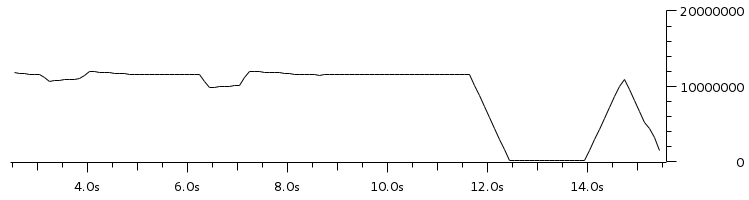
\includegraphics[width=0.85\textwidth]{images/benchmark/bench-1000-1-eth.png}
%    \caption{Example getting tcp throughput graph for specific benchmark test}
%\end{figure}

%\subsubsection{Iptraf-ng}
\newpage
\subsection{Early stress tests}
A early version of the broker provided a console client which produced 
messages per console input. This setup demonstrated that encoding/decoding of a
request worked. Also the different broker layers done their job well.
Later in the construction phase of the broker, tests which repeatedly send
a large amount of requests in short period of time where introduced. This kind
of stress test is very useful to test network related bugs and performance
lacks. The following table lists some of the major issues, that were uncovered: 

\begin{table}[H]
\begin{tabular}{|p{4cm}|p{5cm}|p{6cm}|}
\hline
{\bf Uncovered Issue}                                                                                  & {\bf Cause}                                                                                                                                                                                                                 & {\bf Solution}                                                                                                                                                                                                                                                                                    \\ \hline
Dramatically slowdown after short period of time                                                       & TCP Zero Window - Socket receive buffer of broker full                                                                                                                                                                      & Broker application was to slow in receiving, parsing and handling incoming requests. Threading concept need to be optimized (see \ref{sec:impl-broker-threading}). The process of parsing an incoming request need to be swap out to another thread, so that the network receive thread can reduce socket buffer fast enough. \\ \hline
Parsing from socket error "not enough bytes"  when testing over network interface instead of loopback. & The len argument to the recv system call is merely the upper bound on the received length (e.g. the size of the target buffer); the call may produce less data than asked for & Introduced function which checks if really the exact amount of bytes is read. If not, the recv call is repeat until all requested bytes are present (see details in \ref{sec:impl-broker-socket-receive}).                                                                                                                                              \\ \hline
Throughput drop when producing larger request with nested list                                         & Issue in encoding a request, called runPut on each sub element and appended to a whole.                                                                                                                                     & No appending of parsed sub elements. Restructure encode module by running runPut at latest point in time. This gaves +50\% performance in building requests (see \ref{sec:impl-prot-encoding}).                                                                                                                                      \\ \hline
Very slow performance in persisting messages to the log (file system).                                 & No state and batching at broker side. Each incoming message ended in multiple file accesses which slowed down the whole process.                                                                                                                                & Messages need to be sum up to larger chunks of bytes. After defined period of time or amount of bytes, multiple messages need to be flushed to disk at once (see details of different approaches in \ref{sec:impl-broker-log}).                                                                                                                                      \\ \hline
\end{tabular}
\end{table}
\captionof{table}{Uncovered issues in early stress tests}


\subsection{Profiling}
When dealing with thousands of request per seconds, function with high complexity
can cause terribly bottlenecks. A method to analyze Haskell code for
potentially slow functions is time and allocation profiling provided by GHC.

-- Setup?
-- Results 

\subsection{Producer Benchmark "Effect of Message Batch size"}
The goal of this benchmark is to analyze the network throughput between
producer client and broker system.  The focus lies on the effect of changing
the batch size at producer client to the resulting transmission of bytes per
second. The batch size determines the amount of bytes for which messages will
be packed together and sent to broker as single request for efficiency.
Increasing the batch size requires more memory. The size of a single message is
fixed to 100 bytes, because if is the more interesting case for a messaging system
(generally). It is easy to get good throughput in MB/sec if the messages are
large, but much harder to get good throughput when the messages are small, as
the overhead of processing each message dominates. 

\subsubsection{Conditions}
\begin{table}[H]
\begin{tabular}{|l| p{12cm}|} \hline
{\bf Message Size}   & 100 Bytes \\ \hline
{\bf Batch Size [B]} & 100 | 1000 | 8192 (Kafka benchmarks) | 16384 (Kafka default) \\ \hline
{\bf Tested Clients} &
    \begin{itemize}
        \item Kafka PerformanceProducer 2.10-0.8.2.0 (ref), single threaded
        \item HMB Producer (ref), single threaded
    \end{itemize}\\ \hline
{\bf Tested Brokers} &
    \begin{itemize}
        \item Kafka Broker 2.10-0.8.2.0 (ref), no replication, one partition
        \item HMB Broker, no replication, one partition
    \end{itemize}\\ \hline
{\bf Measurement} & Resulting TCP throughput over a period of 10 seconds, analyzed with
    Wireshark. \\ \hline
{\bf Scenarios} & Producing as much messages as possible from client (left) to broker (right).
    The size of messages batched together varies in defined steps.
    \begin{enumerate}
        \item Kafka Performance Producer -> Kafka Broker
        \item Kafka Performance Producer -> HMB Broker
        \item HMB Produer -> Kafka Broker
        \item HMB Produder -> HMB Broker
    \end{enumerate} \\ \hline
\end{tabular}
\end{table}
\captionof{table}{Benchmark conditions "Effect of Producer Batch size"}

\subsubsection{Results}
\begin{table}[H]
\centering
\begin{tabular}{|l|l|l|l|l|}
\hline
{\bf Benchmark Variable} & \multicolumn{4}{c|}{{\bf Avg. Throughput {[}MB/s{]}}} \\ \hline
Batch Size [Byte]        & Scenario 1       & Scenario 2       & Scenario 3   & Scenario 4   \\ \hline
100                      & 0                & 0                & 30   &           \\ \hline
1000                     & 0                & 0                & 32   &           \\ \hline
8192                     & 0                & 0                & 0    &           \\ \hline
16384                    & 0                & 0                & 0    &           \\ \hline
\end{tabular}
\end{table}
\captionof{table}{Results of benchmark "Effect of Producer Batch size"}

\subsubsection{Conclusion}


\subsection{Producer Benchmark "Effect of Message size"}
The goal of this benchmark is to analyze the network throughput between
producer client and broker system. The focus lies on the effect of changing the
size of a single message to the resulting transmission of bytes per
second. Persisting performance on the broker is not considered in
this benchmark.

\subsubsection{Conditions}
\begin{table}[H]
\begin{tabular}{|l| p{12cm}|} \hline
{\bf Message Size}   & 10 | 100 | 1000 | 10000 | 100000 | Bytes \\ \hline
{\bf Batch Size}     & 12800 \\ \hline
{\bf Tested Clients} &
    \begin{itemize}
        \item Kafka PerformanceProducer 2.10-0.8.2.0 (ref), single threaded
        \item HMB Producer (ref), single threaded
    \end{itemize}\\ \hline
{\bf Tested Brokers} &
    \begin{itemize}
        \item Kafka Broker 2.10-0.8.2.0 (ref), no replication, one partition
        \item HMB Broker, no replication, one partition
    \end{itemize}\\ \hline
{\bf Scenarios} & Producing as much messages as possible from client (left) to broker (right).
    The size of a messages varies in defined steps. The batch size thereby is a fixed value. 
  \begin{enumerate}
        \item Kafka Performance Producer -> Kafka Broker
        \item Kafka Performance Producer -> HMB Broker
        \item HMB Produer -> Kafka Broker
        \item HMB Produder -> HMB Broker
    \end{enumerate} \\ \hline
\end{tabular}
\end{table}
\captionof{table}{Benchmark conditions "Effect of Message size"}

\subsubsection{Results}
\begin{table}[H]
\centering
\begin{tabular}{|l|l|l|l|l|}
\hline
{\bf Benchmark Variable} & \multicolumn{4}{c|}{{\bf Avg. Throughput {[}MB/s{]}}} \\ \hline
Message Size             & Scenario 1       & Scenario 2       & Scenario 3     & Scenario 4 \\ \hline
10 B                     &                  &                  & 0              &           \\ \hline
100 B                    & 0                & 0                & 0              &            \\ \hline
1000 B (1 KB)            & 0                & 0                & 0              &            \\ \hline
10000 B (10 KB)          & 0                & 0                & 0              &            \\ \hline
100000 B (100 KB)        & 0                & 0                & 0              &             \\ \hline
1000000 (1 MB)           & 0                & 0                & 0              &             \\ \hline
\end{tabular}
\end{table}
\captionof{table}{Results of benchmark "Effect of Message size"}

%\subsection{Benchmark "Encode/Decode"}

%\subsection{Network Throughput}
%The socket based communication must not be a bottleneck in a high performance
%broker. A producer should be able to send with near the maximal throughput of
%its local network card, whereas the broker needs to handle the incoming data
%streams as fast as possible. If the limits of a single network connection is
%reached, the next step to improve performance is to balance the data
%stream on multiple replicated brokers.

%To test the network throughput for this thesis, a benchmark producer
%which identify the limits is provided.



%The variance seems to be due to Linux's I/O management facilities that batch
%data and then flush it periodically.
%-> Durchgeführte Tests 

%-> Resultat Network Throuput 

%-> Resultat Writing to the log 
%-> Vergleich Kafka (ref to Blog) 

%\begin{table}[h]
%\begin{tabular}{|c|c|c|c|}
%\hline
%{\bf Request Size (with ReqHeader)} & {\bf Message Size {[}Byte{]}} & {\bf Batch Size} & {\bf \begin{tabular}[c]{@{}c@{}}Avg. Throughput\\ {[}MB/s{]}\end{tabular}} \\ \hline
%150 B                               & 100                           & 1                & 27                                                                         \\ \hline
%1050 B                              & 100                           & 10               & 22                                                                         \\ \hline
%10.050 KB                           & 100                           & 100              & 30                                                                         \\ \hline
%100.050 KB                          & 100                           & 1000             & 32                                                                         \\ \hline
%1 MB                                & 100                           & 10000            & 40                                                                         \\ \hline
%550 B                               & 500                           & 1                & 66                                                                         \\ \hline
%1050 B                              & 500                           & 2                & 81                                                                         \\ \hline
%10.050 B                            & 500                           & 20               & 80                                                                         \\ \hline
%100.050 KB                          & 500                           & 200              & 96                                                                         \\ \hline
%1 MB                                & 500                           & 2000             & 68                                                                         \\ \hline
%1050 B                              & 1000                          & 1                & 104                                                                        \\ \hline
%10.050 B                            & 1000                          & 10               & 110                                                                        \\ \hline
%100.050 KB                          & 1000                          & 100              & 112                                                                        \\ \hline
%1 MB                                & 1000                          & 1000             & 87                                                                         \\ \hline
%10.050 B                            & 10000                         & 1                & 117                                                                        \\ \hline
%100.050 KB                          & 10000                         & 10               & *                                                                          \\ \hline
%1 MB                                & 10000                         & 100              & *                                                                          \\ \hline
%\end{tabular}
%\end{table}


\section{Outlook}
-> What are the next step? 

- Further optimizations 
- Implementation and handling of remaining API's 
- Replication and Integration With Apache Zookeeper 
- Ausbauen von Client API 
-> Open Source 

-> 
- broker results promissing
- very extendable/scalable implementation base and architecture
- with further work one could build the current prototype to an extraordinary
broker system.

As for now, the highlight remains the protocol implementation which has already
been praised by the Haskell community and found its contributors they helped
uncovering minor issues.

